\documentclass[]{report}
\usepackage{ctex}
\usepackage[utf8x]{inputenc}
\usepackage{hyperref}
\usepackage{graphicx}
\usepackage{listings}
\lstset{basicstyle=\sffamily,
keywordstyle=\bfseries,
commentstyle=\rmfamily\itshape,
stringstyle=\ttfamily,
columns=flexible,
numbers=left,
numberstyle=\footnotesize
}

% Title Page
\title{2013-2014学年ISTC技术部算法组工作总结}
\author{李浩成}


\begin{document}
\maketitle

\begin{abstract}
\end{abstract}
\chapter{上半学期}
上半学期主要进行关键算法、\verb|C#|、\verb|OpenCV|、软件工程教学。
\section{13-10-20 组会}
\begin{enumerate}
	\item 开场
	\item 通知事情
	\begin{itemize}
		\item 例会时间
		\item 智慧地球
		\item 奖励措施
	\end{itemize}	
	\item 项目介绍
	\begin{itemize}
		\item 要求:信心,努力
		\item 内容
		\item 各位介绍思路
		\item 分工
		\begin{itemize}
			\item OpenCV
			\item PathFinding
			\item UI
		\end{itemize}
	\end{itemize}	
	\item 注意事项
	\begin{itemize}
		\item 调试笔记
	\end{itemize}
\end{enumerate}

\section{13-10-26 组会}
\begin{enumerate}
	\item 通知
	\begin{itemize}
		\item 加微信主页 \verb|xjtuistc|
		\item 冬游
	\end{itemize}
	\item 安装 \verb|Microsoft Visual Studio 2013 Utimate|
	\item 每个人介绍工作情况
	\item 介绍寻路算法
	\begin{itemize}
		\item \verb|DFS|
		\item \verb|Dijkstra|
		\item \verb|A*|
		\item \verb|SPFA|
	\end{itemize}
\end{enumerate}

\section{13-11-03 组会}
\begin{enumerate}
	\item 创建 \verb|ISTC Smart Tech Community|
	\item \verb|OpenCV| 基本数据结构
	\lstinputlisting[language=C++]{CODE/CVStruct.hpp}
	\item \verb|OpenCV| 窗口句柄
	\item 侵蚀算法
	\item 软件推荐 
	\begin{itemize}
	\item Notepad++
		
	\href{http://notepad-plus-plus.org/zh/download/v6.5.1.html}{Notepad++ v6.5.1}
	\end{itemize}
	
\end{enumerate}
	\subsection{13-11-04 资讯}
		纪念印度数学家 "人脑计算机" Shakuntala Devi 84岁诞辰。
	\subsection{13-11-05 资讯}
		纪念美国工业设计先锋 Raymond Loewy 120岁诞辰。
		
		\href{www.raymondloewy.com/}{The Official Site of Raymond Loewy}‎
		
	\subsection{13-11-06 资讯}
		Winter is coming, SDN as well. Here's one take on what it all means.
		
		\href{http://ow.ly/qy9Ei}{Software-defined networking explained - Network World}
	
	\subsection{13-11-08 资讯}
		Nokia camera app is named as Nokia Smart Cam.
		
\section{13-11-09 组会}
\begin{enumerate}
	\item 软件工程
		丰田凯美瑞暴冲事件系统分析。
	\item \verb|C#| 基本语法教学
\begin{figure}
\centering
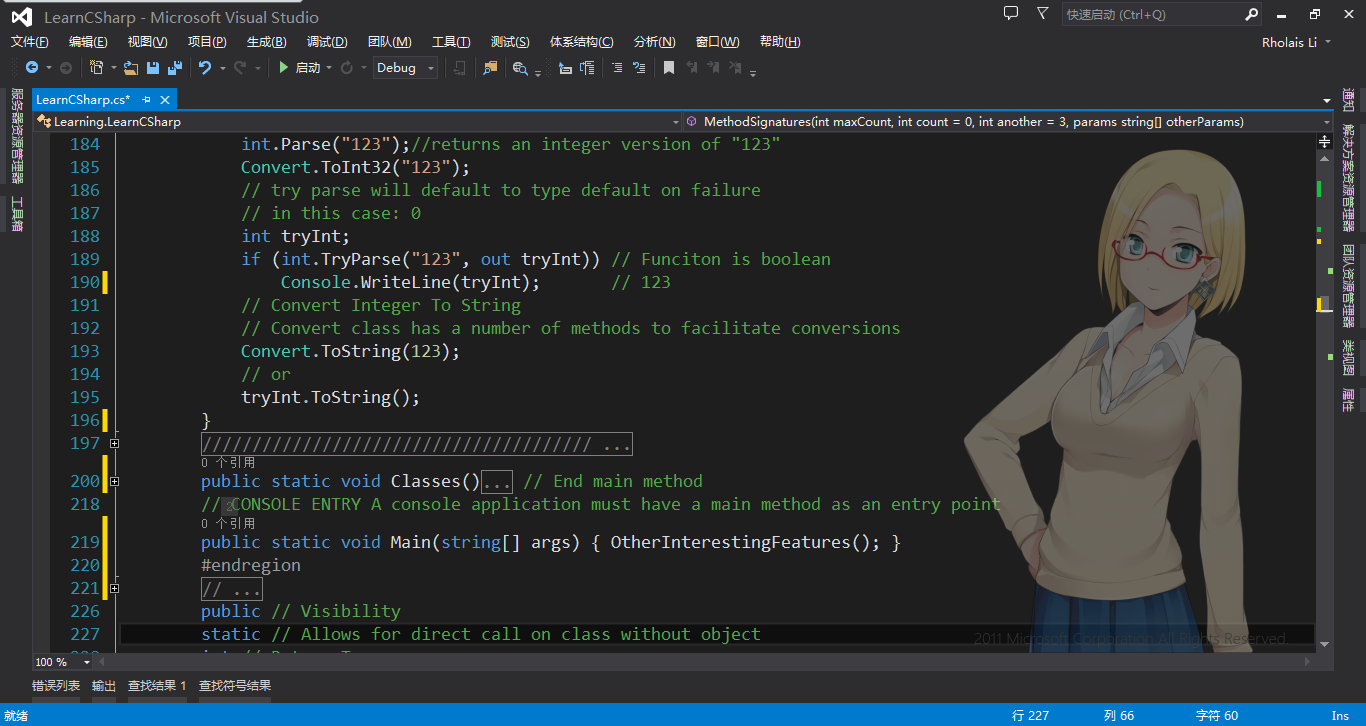
\includegraphics[width=1\linewidth]{./PIC/LearnCSharp}
\caption{CSharp 基本语法教学}
\label{fig:LearnCSharp}
\end{figure}
\end{enumerate}

\section{13-11-17 组会}
\begin{enumerate}
	\item \verb|C# Windows Form|控件
	\begin{itemize}
		\item[Button] 按钮
		\item[Label] 标签
		\item[TextBox] 文本框
		\item[CheckBox] 多选框
		\item[LinkLabel] 链接
		\item[TabPage] 标签页
	\end{itemize}
\begin{figure}
\centering
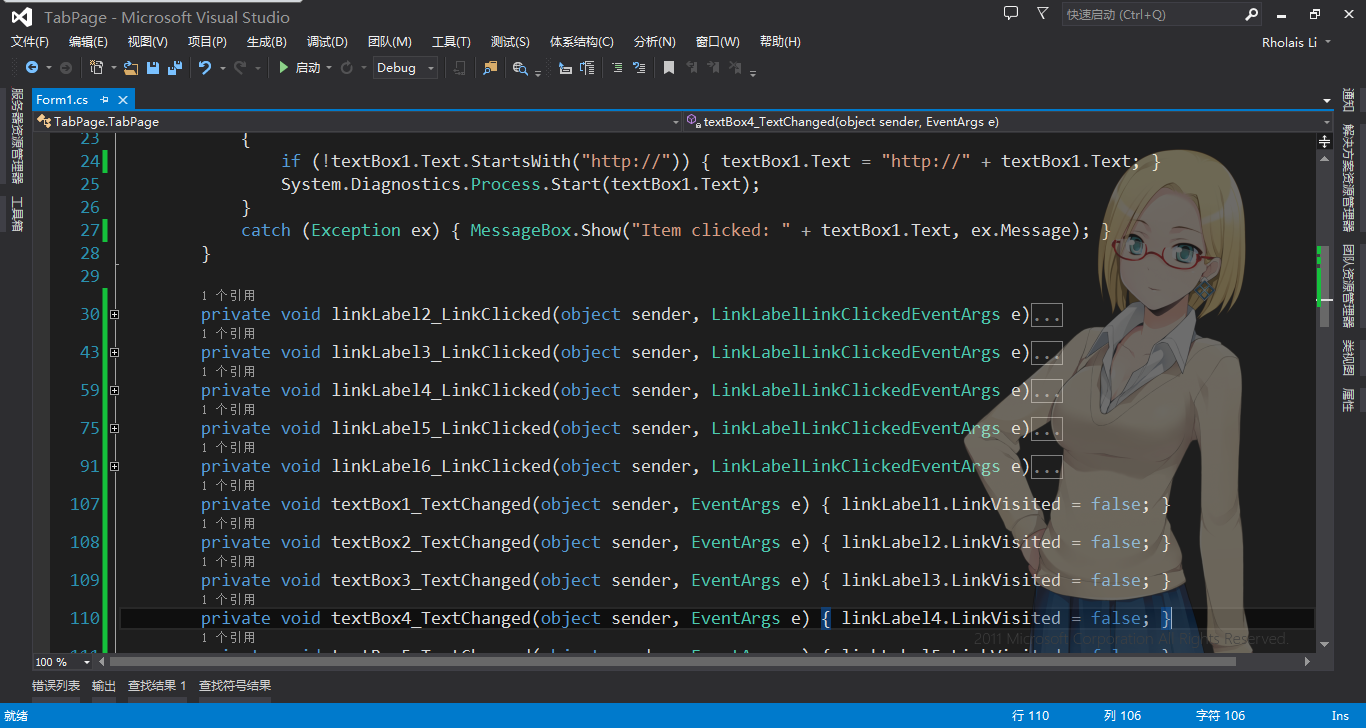
\includegraphics[width=1\linewidth]{./PIC/TabPage}
\caption{CSharp Windows Form控件:标签页教学}
\label{fig:TabPage}
\end{figure}
\begin{figure}
\centering
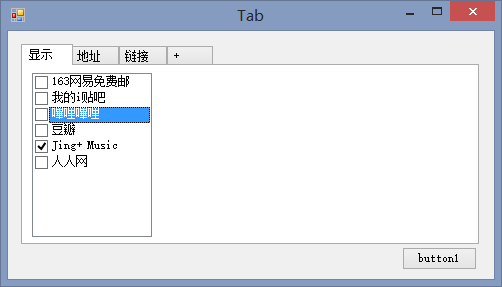
\includegraphics[width=0.7\linewidth]{./PIC/TabPageO}
\caption{CSharp Windows Form控件:标签页运行结果}
\label{fig:TabPageO}
\end{figure}
\end{enumerate}

\section{13-11-23 组会}
\begin{enumerate}
	\item \verb|C# Windows Form|控件
	\begin{itemize}
		\item[ComboBox] 组合框
		
			\verb|ComboBox| 显示与一个 \verb|ListBox| 组合的文本框,使用户可以从列表中选择项,也可以输入新值。\verb|DropDownStyle| 属性指定是否始终显示列表或者列表是否显示在下拉列表中。
		\item[ListBox] 下拉菜单
		
			\verb|ListBox| 控件使您得以向用户显示一列项,用户可通过单击选择这些项。 \verb|ListBox| 控件可使用 \verb|SelectionMode| 属性提供单项选择或多重选择。
		\item[RatioButton] 选项按钮
		
			\verb|RadioButton| 控件可以显示文本、\verb|Image| 或同时显示两者。
			当用户选择一个组内的一个选项按钮(也称作单选按钮)时,其他选项按钮自动清除。 给定容器(如 \verb|Form|)中的所有 \verb|RadioButton| 控件构成一个组。 若要在一个窗体上创建多个组,请将每个组放在它自己的容器(例如 \verb|GroupBox| 或 \verb|Panel| 控件)中。
	\end{itemize}
\begin{figure}
\centering
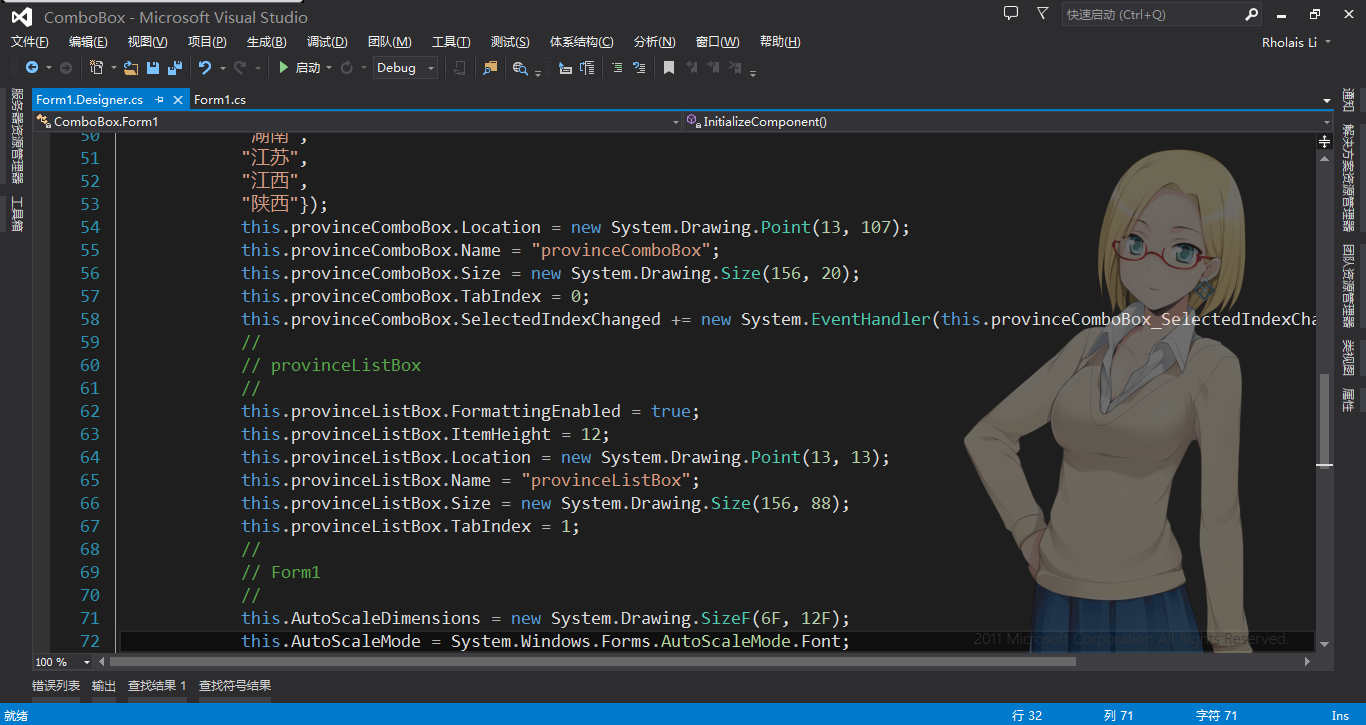
\includegraphics[width=1\linewidth]{./PIC/ComboBox}
\caption{CSharp Windows Form控件:组合框教学}
\label{fig:ComboBox}
\end{figure}
\begin{figure}
\centering
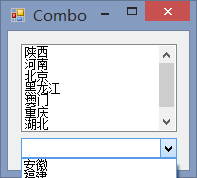
\includegraphics[width=0.7\linewidth]{./PIC/ComboBoxO}
\caption{CSharp Windows Form控件:组合框运行结果}
\label{fig:ComboBoxO}
\end{figure}
\end{enumerate}
	\subsection{13-11-24 资讯}
		\href{http://rrurl.cn/fCQ7bT}{提问的智慧}
\section{13-11-31 组会}
\begin{enumerate}
	\item \verb|C# GDI+|
	\begin{itemize}
		\item 绘制图片
\begin{figure}
\centering
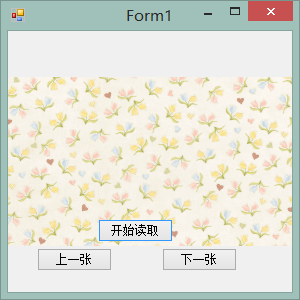
\includegraphics[width=0.7\linewidth]{./PIC/DengPic0}
\caption{绘制图片部员作品:图片浏览器:首页}
\label{fig:DengPic0}
\end{figure}
\begin{figure}
\centering
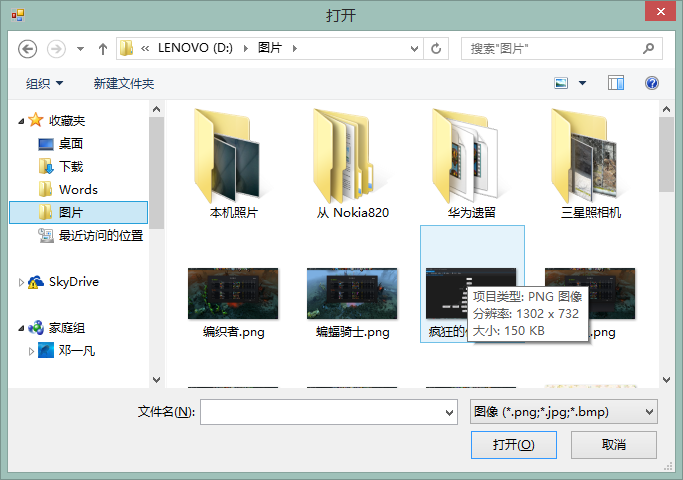
\includegraphics[width=0.7\linewidth]{./PIC/DengPic1}
\caption{绘制图片部员作品:图片浏览器:打开图片}
\label{fig:DengPic0}
\end{figure}
\begin{figure}
\centering
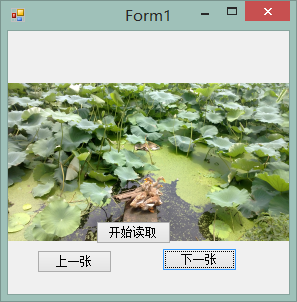
\includegraphics[width=0.7\linewidth]{./PIC/DengPic2}
\caption{绘制图片部员作品:图片浏览器:显示界面}
\label{fig:DengPic0}
\end{figure}
\begin{figure}
\centering
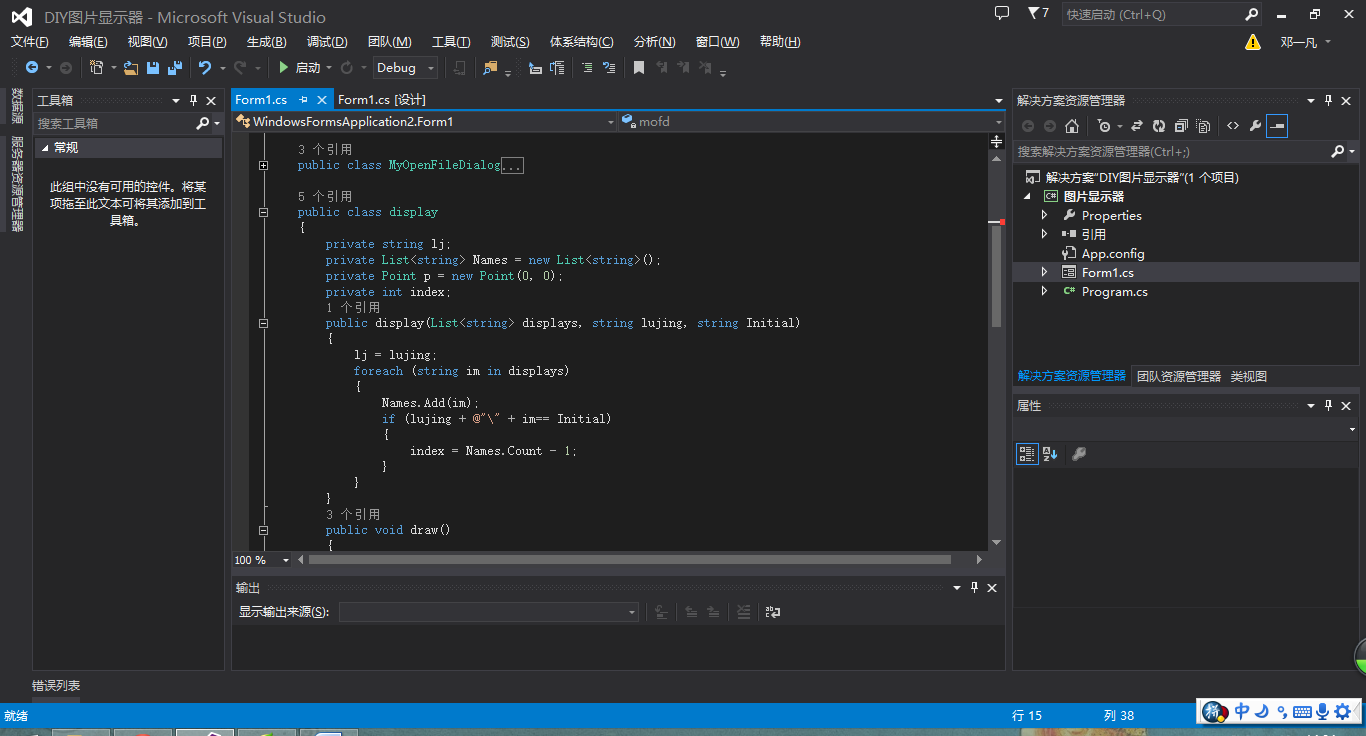
\includegraphics[width=1\linewidth]{./PIC/DengPic3}
\caption{绘制图片部员作品:图片浏览器:代码}
\label{fig:DengPic0}
\end{figure}
	\end{itemize}
\end{enumerate}
\section{13-12-06 组会}
\begin{enumerate}
	\item \verb|C# GDI+|
	\begin{itemize}
		\item 绘制几何图形
\begin{figure}
\centering
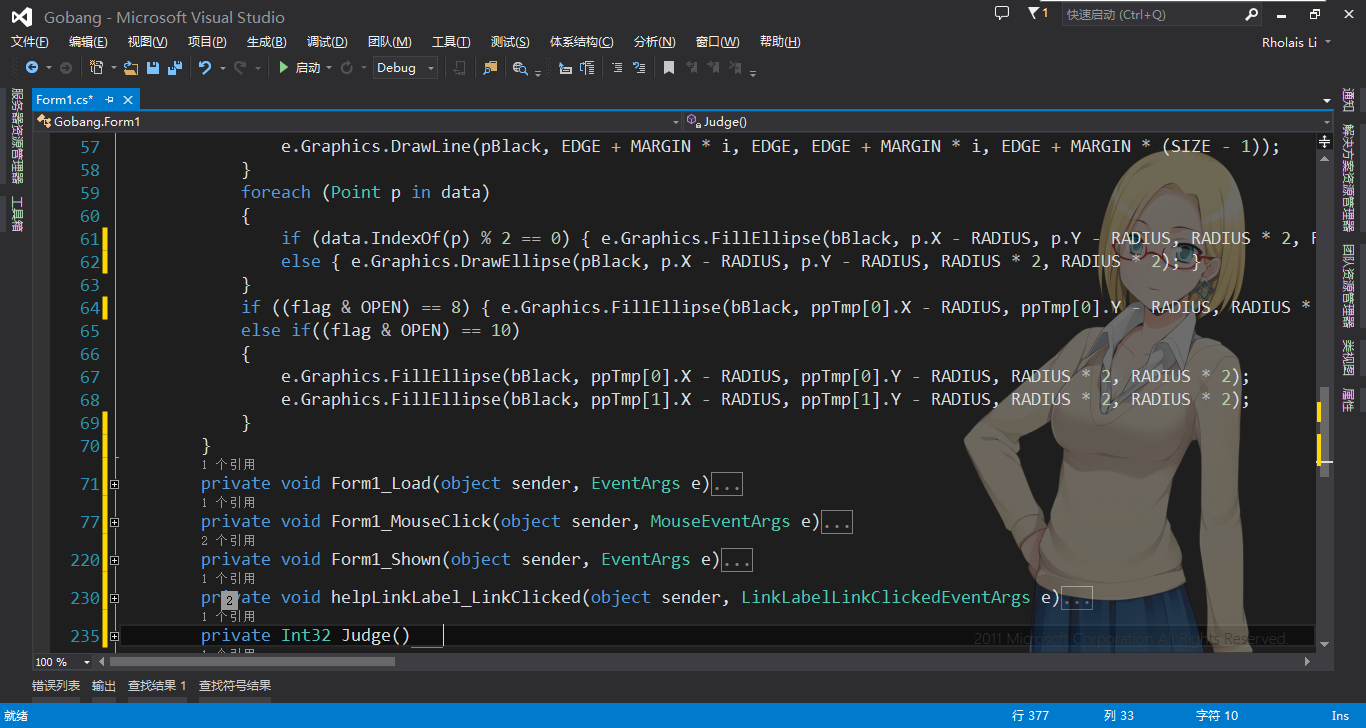
\includegraphics[width=1\linewidth]{./PIC/Gobang}
\caption{CSharp GDI+:绘制几何图形教学}
\label{fig:ComboBox}
\end{figure}
\begin{figure}
\centering
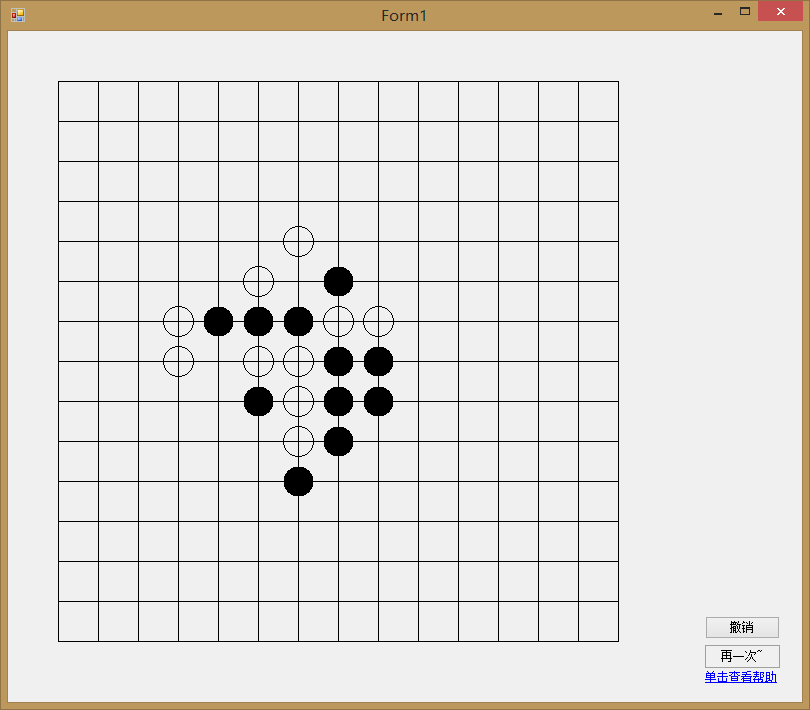
\includegraphics[width=0.7\linewidth]{./PIC/GobangO}
\caption{CSharp GDI+:绘制几何图形运行结果}
\label{fig:GobangO}
\end{figure}
	\end{itemize}
\end{enumerate}
	\subsection{13-12-10 资讯}
			\href{http://notepad-plus-plus.org/zh/download/v6.5.2.html}{Notepad++ v6.5.2}
\section{13-12-14 组会}
\begin{enumerate}
	\item 使用\verb|C#|引用\verb|C++ Dynamic Link Library|
\begin{figure}
\centering
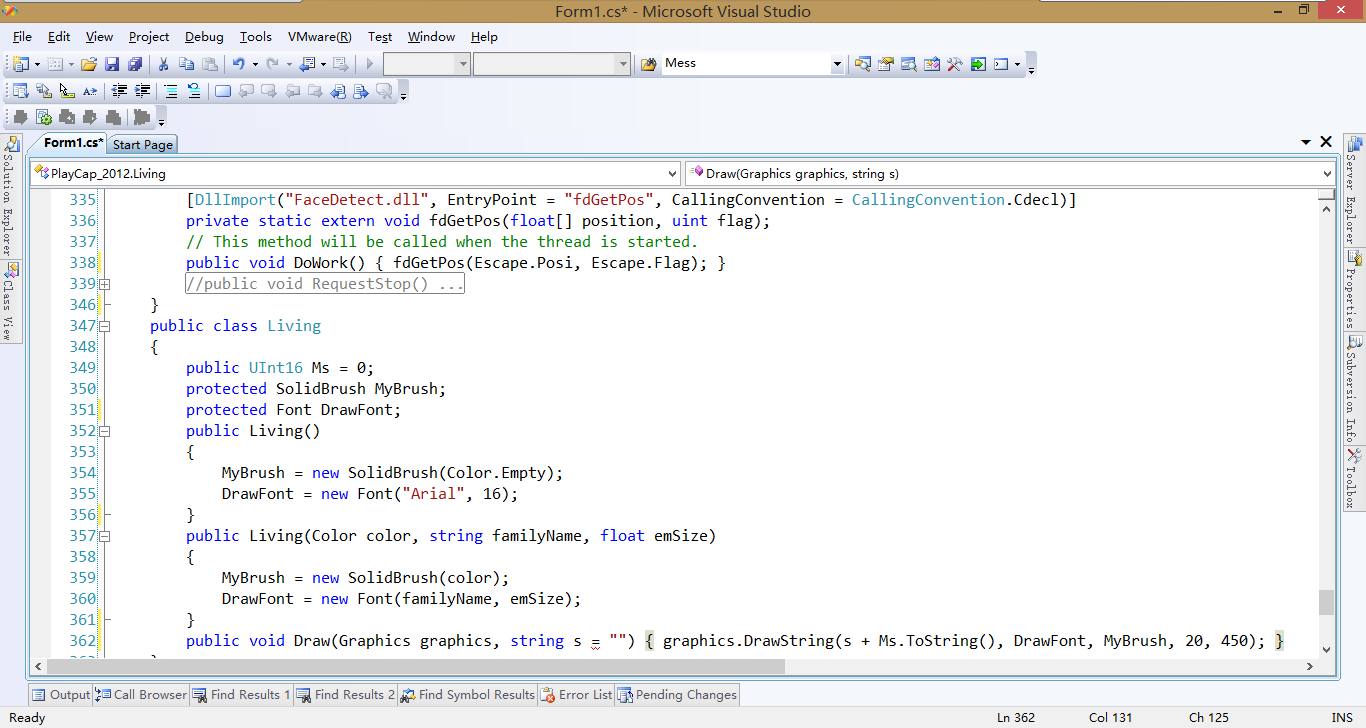
\includegraphics[width=1\linewidth]{./PIC/PlayCap}
\caption{CSharp 引用 DLL:教学}
\label{fig:PlayCap}
\end{figure}
\begin{figure}
\centering
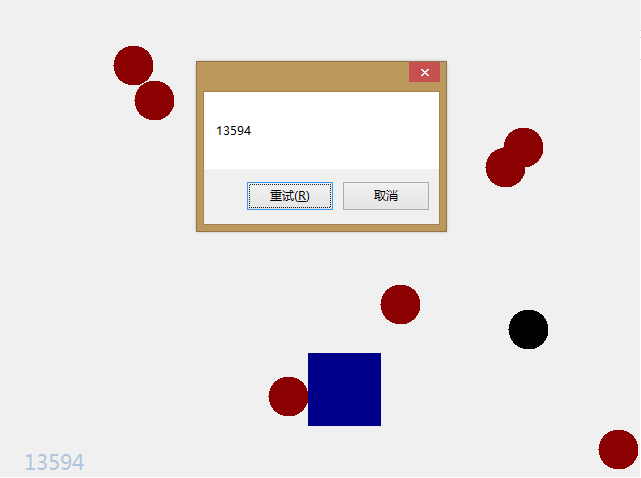
\includegraphics[width=0.7\linewidth]{./PIC/PlayCapO}
\caption{CSharp 引用 DLL:运行结果}
\label{fig:PlayCapO}
\end{figure}
\end{enumerate}
	\subsection{13-12-31 资讯}
		\href{http://notepad-plus-plus.org/zh/download/v6.5.3.html}{Notepad++ v6.5.3}
\chapter{下半学期}
\section{14-02-02 组会}
\begin{enumerate}
		\item \verb|C# Windows Form|控件
		\begin{itemize}
			\item[Timer] 计时器
			\verb|Timer| 用于以用户定义的事件间隔触发事件。 \verb|Windows| 计时器是为单线程环境设计的,其中,\verb|UI| 线程用于执行处理。 它要求用户代码有一个可用的 \verb|UI| 消息泵,而且总是在同一个线程中操作,或者将调用封送到另一个线程。
			使用此计时器时,请使用 \verb|Tick| 事件执行轮询操作,或在指定的时间内显示启动画面。 每当 \verb|Enabled| 属性设置为 \verb|true| 且 \verb|Interval| 属性大于 $0$ 时,将引发 \verb|Tick| 事件,引发的时间间隔基于 \verb|Interval| 属性设置。
			此类提供用于设置时间间隔以及启动和停止计时器的方法。
		\end{itemize}
\end{enumerate}
	\subsection{14-02-08 资讯}
		\href{http://www.java.net/download/jdk8/archive/b128/binaries/jdk-8-fcs-bin-b128-windows-x64-01_feb_2014.exe}{JDK 8 build b128}
		
		JDK 8 的候选发行版本终于来了,这是JDK 8 的首个RC 版本,该版本代号为Build 128。
\section{14-03-30 组会}
\begin{enumerate}
	\item 使用逆波兰表达式进行科学计算。
\begin{figure}
\centering
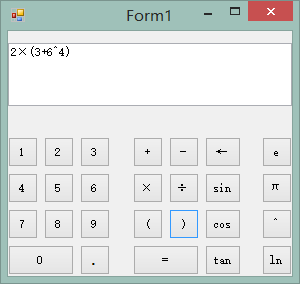
\includegraphics[width=0.7\linewidth]{./PIC/CalcP0}
\caption{科学计算器逆波兰表达式版:输入算式}
\label{fig:CalcP0}
\end{figure}
\begin{figure}
\centering
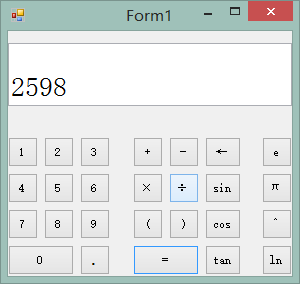
\includegraphics[width=0.7\linewidth]{./PIC/CalcP1}
\caption{科学计算器逆波兰表达式版:输出结果}
\label{fig:CalcP1}
\end{figure}
\begin{figure}
\centering
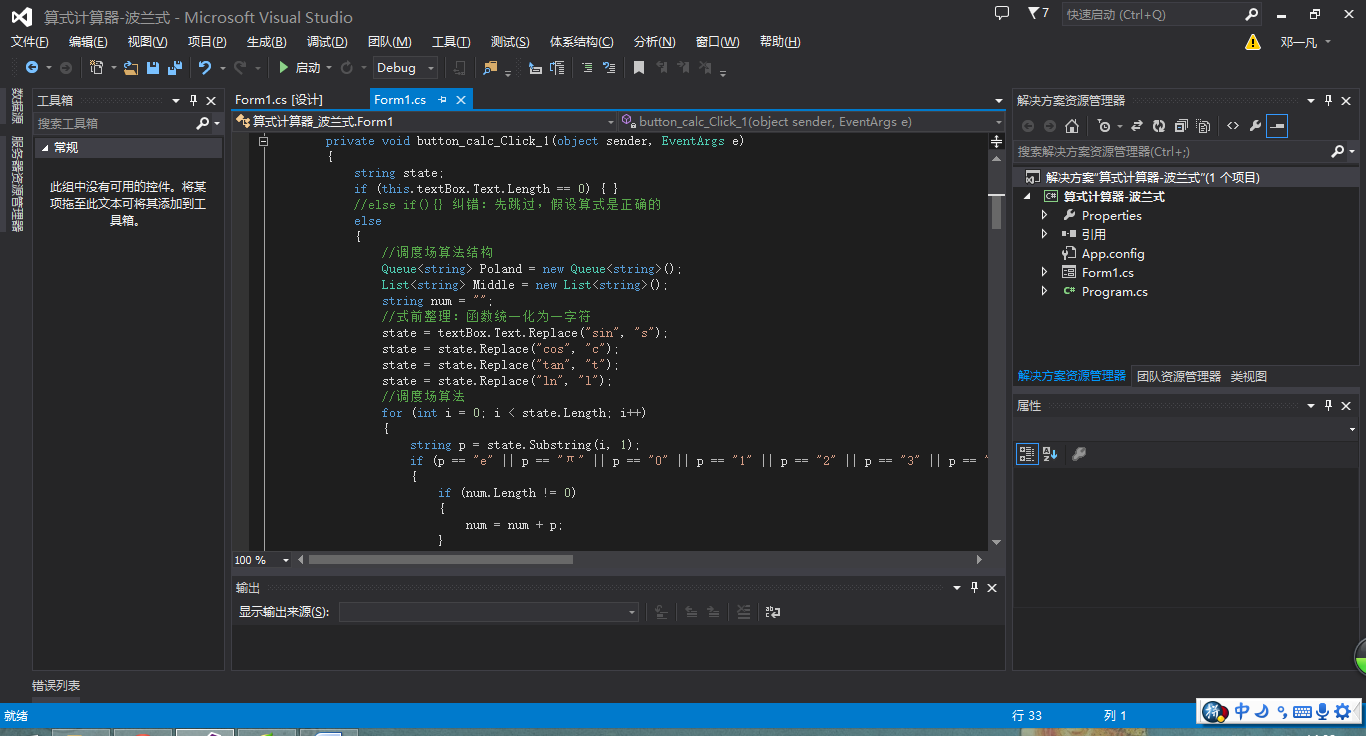
\includegraphics[width=1\linewidth]{./PIC/CalcP2}
\caption{科学计算器逆波兰表达式版:代码}
\label{fig:CalcP2}
\end{figure}
\end{enumerate}
\section{14-04-06 组会}
\begin{enumerate}
	\item 完成科学计算器项目,提交"葡萄城杯"比赛
\begin{figure}
\centering
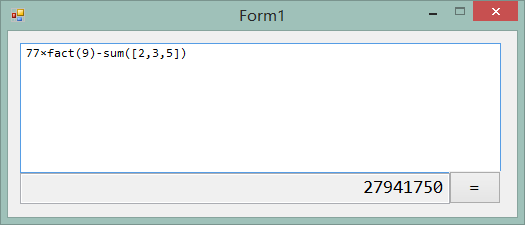
\includegraphics[width=0.7\linewidth]{./PIC/CalcEC0}
\caption{科学计算器最终参赛版:运算实例甲}
\label{fig:CalcEC0}
\end{figure}
\begin{figure}
\centering
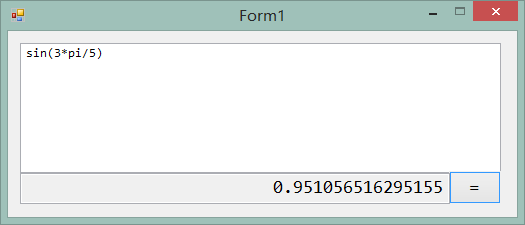
\includegraphics[width=0.7\linewidth]{./PIC/CalcEC1}
\caption{科学计算器最终参赛版:运算实例乙}
\label{fig:CalcEC1}
\end{figure}
\begin{figure}
\centering
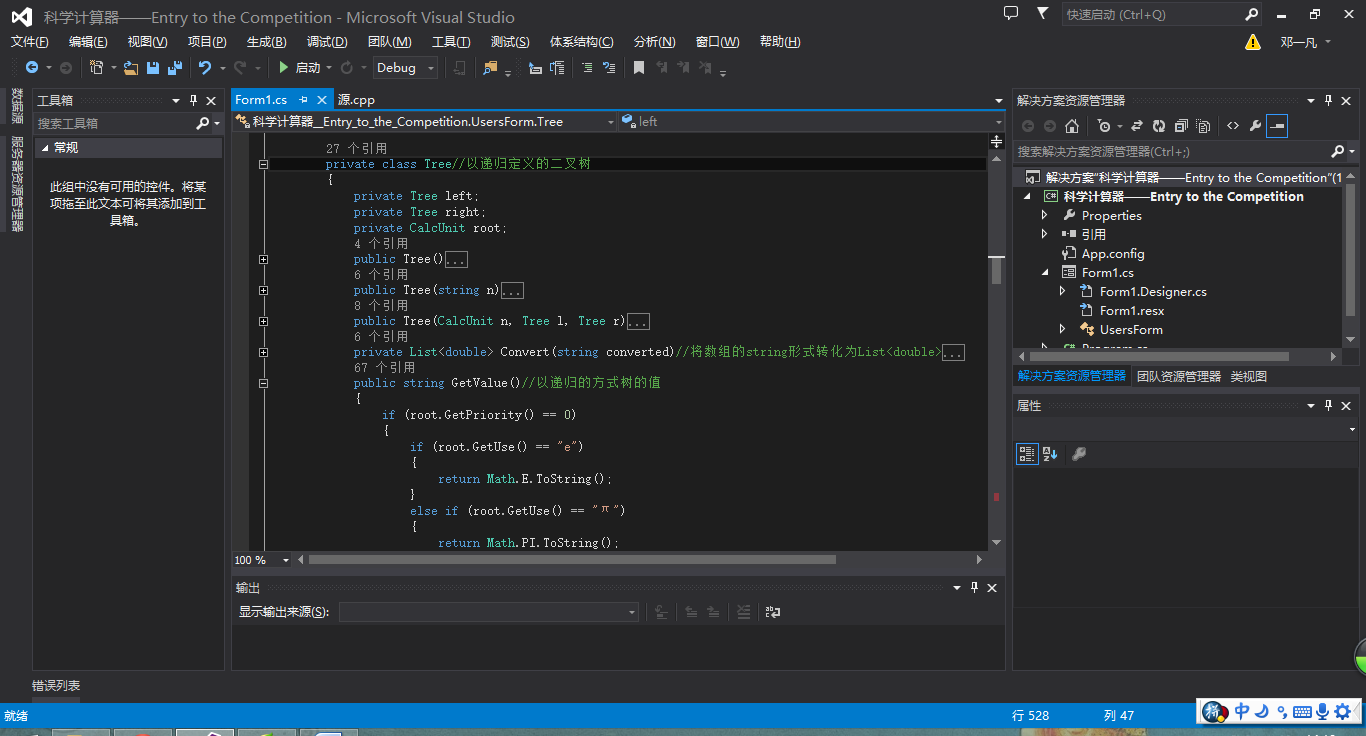
\includegraphics[width=1\linewidth]{./PIC/CalcEC2}
\caption{科学计算器最终参赛版:代码}
\label{fig:CalcEC2}
\end{figure}

\end{enumerate}	
\section{14-04-13 讲座}
\begin{enumerate}
	\item \LaTeX 降龙十八掌\ 文字排版撒手锏
	\begin{enumerate}
		\item \LaTeX 历史
		\item \LaTeX 适合做什么?
		\item \LaTeX 不适合做什么?
		\item \LaTeX 思想
		\item \LaTeX 套件安装方法以及资源列表
		\item \verb|*.tex|文件结构
		\item \LaTeX 中常用宏包
		\item \verb|*.tex|导言区
		\item \LaTeX 环境、语法、段落、目录、符号等……
	\end{enumerate}
\end{enumerate}
	\subsection{14-04-16 资讯}
		\href{http://www.openhw.org/bbs/article_1237_523288.html}{懒兔子的ZedBoard学习手记}
	\subsection{14-04-17 资讯}
		热门虚拟化软件公司\verb|VMware|发布\verb|VMware Workstation 10.0.2|虚拟机最新维护版,版本号也升级至\verb|10.0.2.1744117|,继续支持简体中文,无需第三方的汉化包了。本次\verb|VMware Workstation 10.0.2|继续修复已知问题,提升性能。
\section{14-04-27 组会}
\begin{enumerate}
	\item 开启雷电项目
	\begin{itemize}
		\item 时间控制框架
		\item 关键类
		\item 模型资源文件
\begin{figure}
\centering
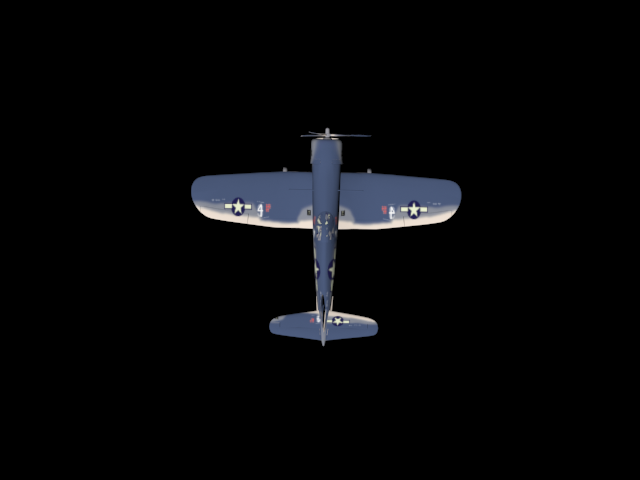
\includegraphics[width=0.7\linewidth]{./PIC/1}
\caption{雷电项目资源文件:仰视图}
\label{fig:1}
\end{figure}
\begin{figure}
\centering
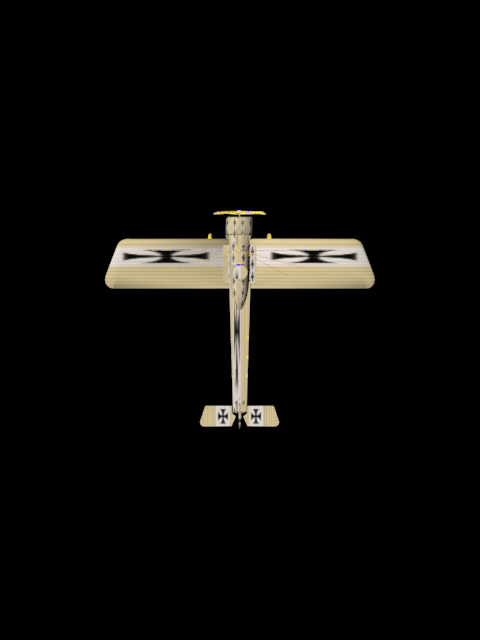
\includegraphics[width=0.7\linewidth]{./PIC/3}
\caption{雷电项目资源文件:俯视图}
\label{fig:3}
\end{figure}
	\end{itemize}
\end{enumerate}
	\subsection{14-04-30 资讯}
		游戏开发生态系统 \verb|Unity| 下载链接:\href{http://netstorage.unity3d.com/unity/UnitySetup-4.3.4.exe}{netstorage.unity3d.com/unity/UnitySetup-4.3.4.exe}
	\subsection{14-05-05 资讯}
		\verb|SW_DVD5_Office_Professional_Plus_2013_64|下载链接: \href{http://pan.baidu.com/s/1hqgLGR6}{pan.baidu.com/s/1hqgLGR6} 密码: u125
	\subsection{14-05-19 资讯}
		\href{http://notepad-plus-plus.org/zh/download/v6.6.3.html}{Notepad++ 6.6.3 released}
	\subsection{14-05-21 资讯}
		纪念英国早期化石收集者及古生物学家 Mary Anning 诞辰 215 周年.
		大体来说,Mary Anning 的发现是生物会灭绝的关键证据。在她的时代,人们广泛的认为生物是不会灭绝的。任何古怪的发现都被认为是地球上尚未被人类发现的生物所造成的。Mary Anning 发现的奇异化石对于这种论调是沉重的打击,也让人类真正理解地质时代早期的真实情况。
\section{14-05-25 组会}
	如何让 \TeX 更有威力
	\subsection{14-06-01 资讯}
		庆祝六一儿童节!
	\subsection{14-06-02 资讯}
		Happy Dragon Boat Festival!
	\subsection{14-06-04 资讯}
		\href{http://notepad-plus-plus.org/zh/download/v6.6.4.html}{Notepad++ 6.6.4 Tiananmen June Fourth Incident Edition}
	\subsection{14-06-06 资讯}
		Honinbo Shusaku's 185th Birthday.
\section{14-06-08 组会}
	聚餐~
	\subsection{14-06-10 资讯}
		\href{http://cdn.winscp.net/files/winscp554setup.exe}{Upgrade to WinSCP 5.5.4}
	\subsection{14-06-13 资讯}
		\href{http://notepad-plus-plus.org/zh/download/v6.6.6.html}{Notepad++ 6.6.6 Friday the 13th Edition}
	\subsection{14-06-15 资讯}
		England vs Italy
\section{14-06-24 部门会议}
\begin{enumerate}
	\item 换届
	\item \href{http://notepad-plus-plus.org/zh/download/v6.6.7.html}{Notepad++ 6.6.7 released}
\end{enumerate}
	\subsection{14-06-25 资讯}
		\href{http://blog.qt.digia.com/blog/2014/06/25/qt-5-3-1-released/}{Qt 5.3.1 Released}
\section{14-06-29 部门会议}
	聚餐。
	\subsection{14-07-01 资讯}
		\href{http://www.vmware.com/cn/support/support-resources/pubs/ws_pubs/workstation-1003-release-notes.html}{VMware Workstation 10.0.3 发行说明}
\end{document}          
